\section{Antrieb}
\subsection{Motoren}
Angetrieben wird das Luftkissenboot von zwei \textbf{Hacker A200-6} Elektromotoren mit einer Dauerleistung von jeweils $10\,\mathrm{kW}$.\\
\begin{figure}[h]
    \centering
    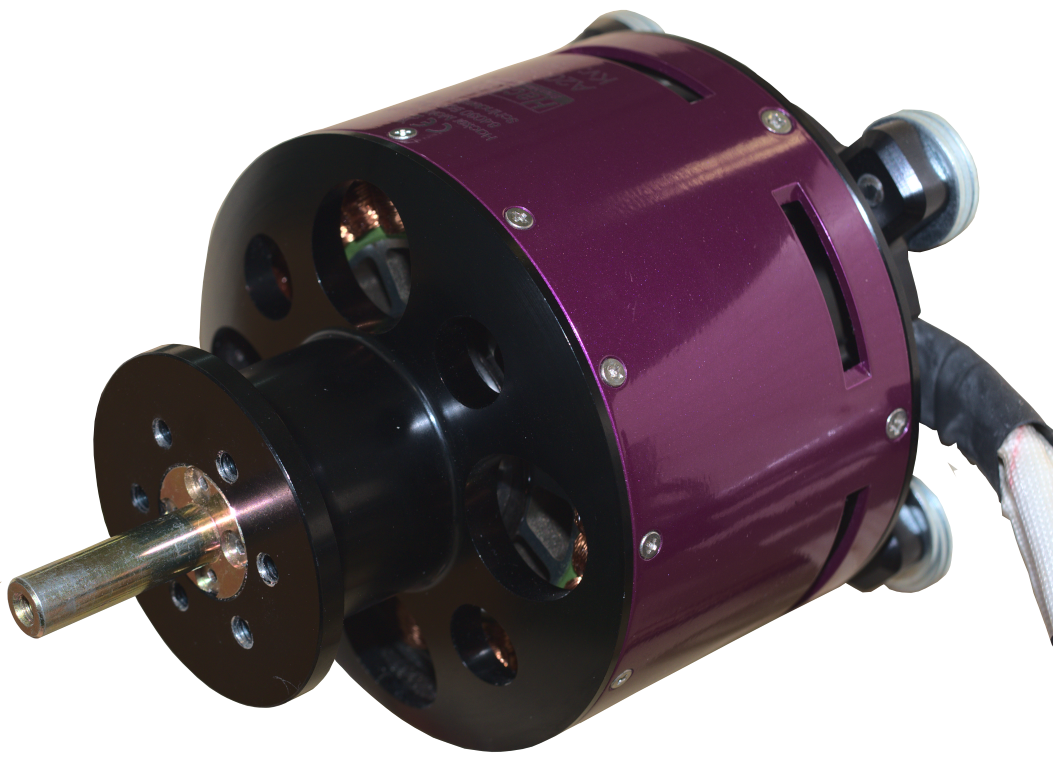
\includegraphics[width=0.55\textwidth]{Fotos/Motor.png}
    \caption{Hacker A200 Elektromotor}
\end{figure}

Konkret weisen die Motoren folgende Leistungsdaten auf:\\
\begin{table}[h]
    \centering
    \begin{tabular}{|c|c|}
        \hline
        Parameter & Wert\\\hline
        Leistung & $10\,\mathrm{kW}$ ($15\,\mathrm{kW}$ max 15 sec.)\\
        Leerlaufstrom ($8.4\,\mathrm{V}$) & $5.1\,\mathrm{A}$\\
        Innenwiderstand & $0.011\,\mathrm{\Omega}$\\
        Polzahl & 20 \\
        empf. Timing & $22^\circ$\\
        Leerlaufdrehzahl&$151\,\mathrm{U/min^{-1}/V}$\\\hline

    \end{tabular}
    \caption{Hacker A200 Leistungsdaten}
\end{table}

\newpage
\subsection{Propeller}
\subsubsection{Zur Erzeugung des Vorschubes}
Hierfür kommt ein zwei blättriger XOAR Elektro Flugzeug-Propeller 28 x 12 Zoll zum Einsatz.

\begin{figure}[h]
    \centering
    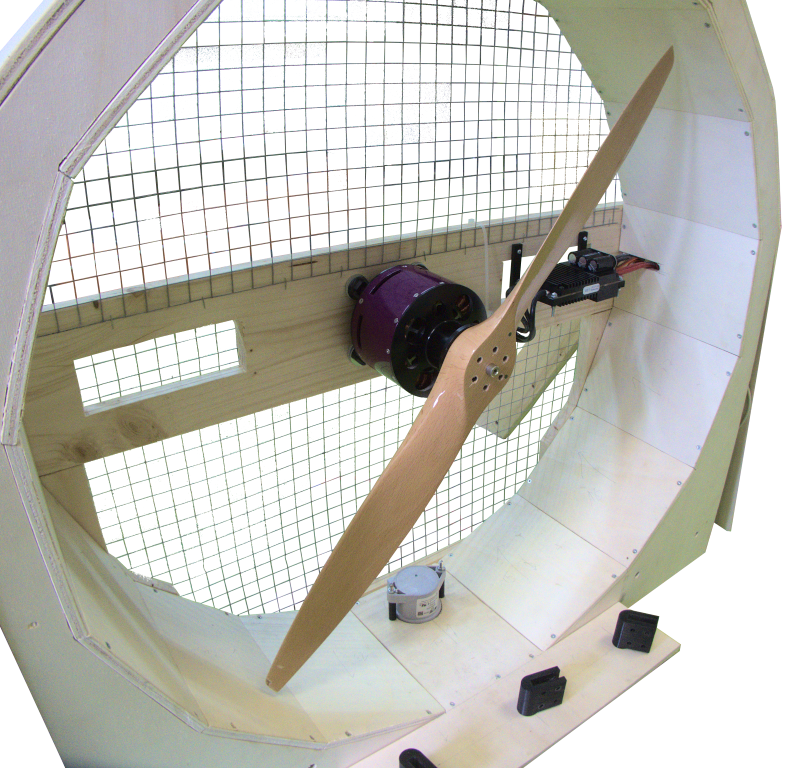
\includegraphics[width=0.8\textwidth]{Fotos/Propeller_Hinten.png}
    \caption{Hinterer Propeller}
\end{figure}

\newpage
\subsubsection{Zur Erzeugung des Auftriebes}
Um das Luftkissen, auf dem das Boot zu schweben beginnt, erzeugen zu können, wurden zwei, drei blättrige, XOAR Elektro Flugzeug-Propeller 28 x 10 Zoll verwendet.  
\begin{figure}[h]
    \centering
    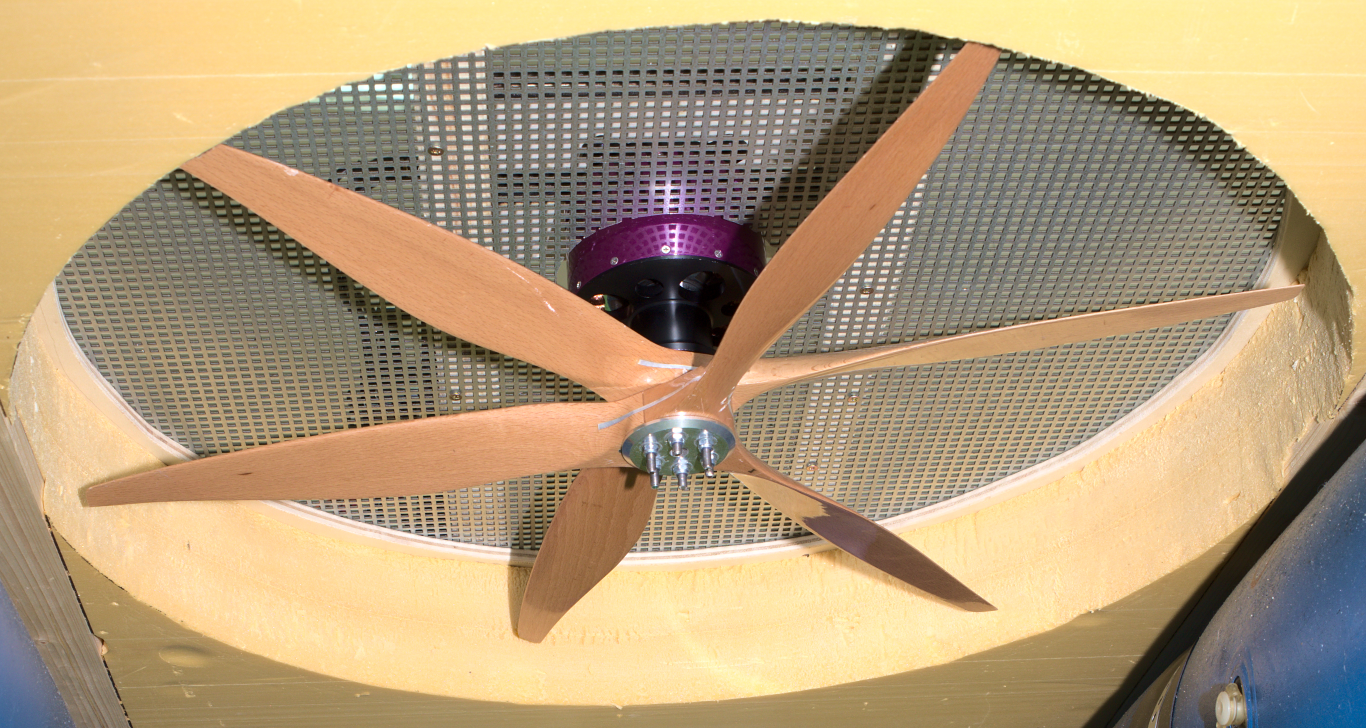
\includegraphics[width=0.9\textwidth]{Fotos/Propeller_unten.png}
    \caption{Unterer Propeller}
\end{figure}

Diese sind $60^\circ$ zueinander versetzt, wodurch die effektive Blattzahl auf sechs erhöht wird, 
um das Entweichen der Luft zurück nach oben hin zu verhindern.


\newpage

\subsection{Motorregler}
Die Ansteuerung der Motoren übernimmt der dafür empfohlene \textbf{MasterSpin 220 Pro OPTO}.
Hierbei handelt es sich um einen Brushless-DC Regler, welcher einen maximalen Dauerstrom von $220\,\mathrm{A}$ aufweist.
\begin{figure}[h]
    \centering
    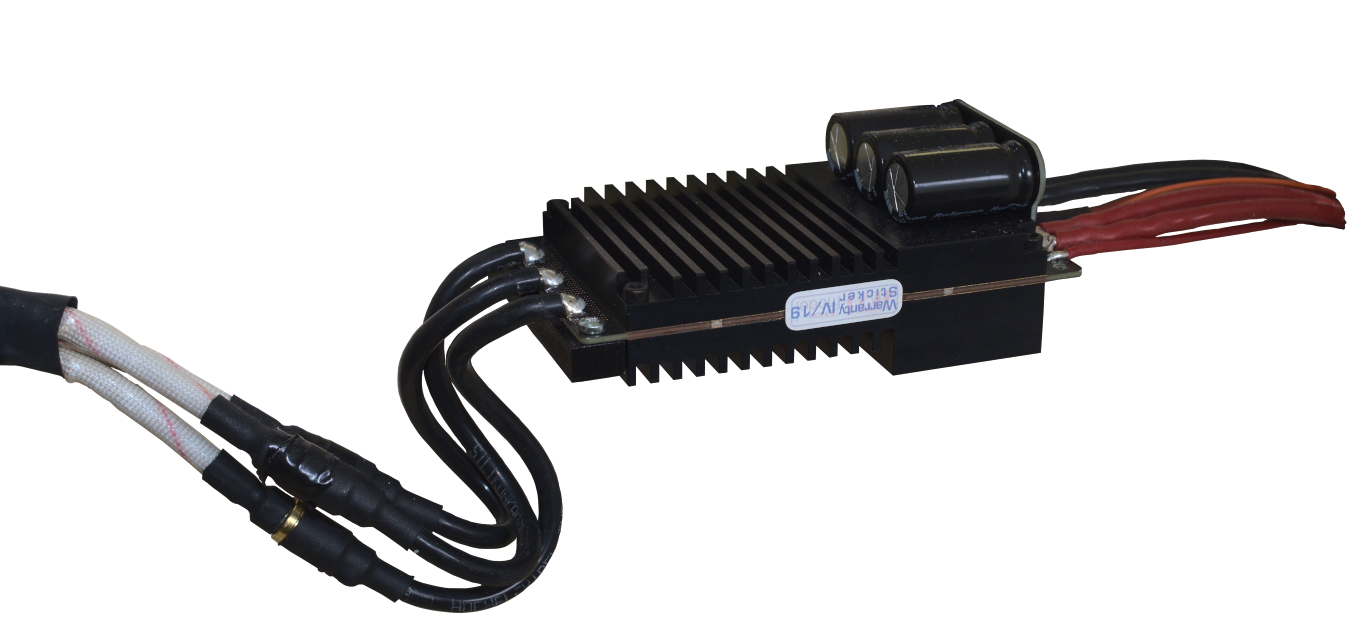
\includegraphics[width=0.9\textwidth]{Fotos/MasterSpin_ohne_Halter.png}
    \caption{MasterSPIN 220 Pro OPTO}
\end{figure}
\subsubsection*{Parametrierung durch JetiBox}
Um den Regler auf unsere Bedürfnisse parametrieren zu können, wurde eine sogenannte "JetiBox" verwendet.
\begin{figure}[h]
    \centering
    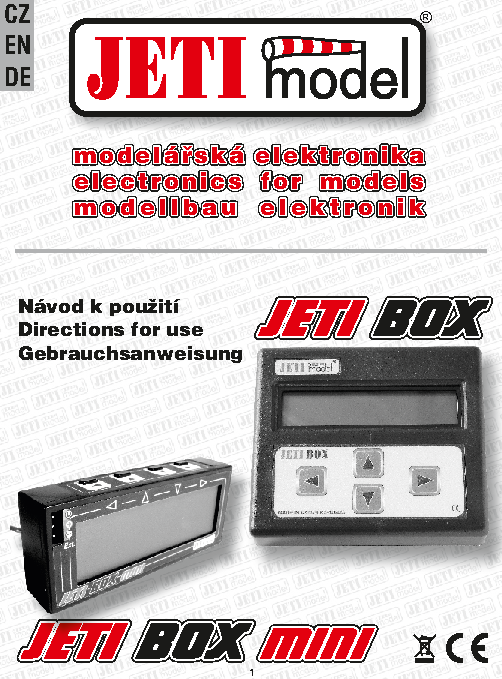
\includegraphics[width=0.5\textwidth]{Fotos/JetiBox.png}
    \caption{Jetibox}
\end{figure}
\newpage
Um in das Konfigurationsmenü des Reglers zu gelangen, muss die JetiBox am kürzeren der beiden 3-poligen Kabeln des MasterSpin 220 PRO OPTO (jenes mit dem roten Stecker) angeschlossen werden, 
während das PWM-Kabel (länger \& schwarzer Stecker) nicht verbunden ist.\\

Konkret wurden folgende Einstellungen getroffen:\\
\begin{table}[h]
\centering
\begin{threeparttable}
    
    \begin{tabular}{|l|l|}
    \hline
     Menüpunkt & getroffene Einstellung \\\hline
     Temp. Protection & $90\,^\circ\,\textrm{C}$\\
     Brake & Hard 70/100/0,5s\\
     Operation Mode & Fast Response\\
     Autorotation & OFF\\
     Timing & $22^\circ$\\
     Frequency & 8 kHz\\
     Acceleration & 0-100\% 5,0 s\\
     Accumulator Type & Li-Ion/Pol/Fe\\
     Number of Cells & Li-XX 14\\
     Li-XX Cut OFF & V Per Cell 3.2\\
     Off Voltage Set & 44,75 V\\
     Cut OFF & Slow Down\\
     Initial Point & AUTO\\
     END Point & 2.05 ms / 2.15 ms \tnote{1}\\
     AutoInc.END Point & OFF(FIX)\\
     Throttle Curve & Linear\\
     Rotation & Left \tnote{2}\\
     Start-up Power & Auto\\
     Setting th. R/C & OFF\\\hline
    \end{tabular}
    \begin{tablenotes}\footnotesize 
        \item[1] 2.15 ms zur Begrenzung der Motorleistung auf \\$\approx 90\%$
        \item[2] Abhängig von der Verkabelung des Motors 
        \end{tablenotes}
    \end{threeparttable}
    \caption{Durch JetiBox am Regler konfigurierte Parameter}
\end{table}

Eine genauere Beschreibung der einzelnen Parameter findet sich in der Anleitung des MasterSpin 220 Pro OPTO's im \autoref{sec:Master_Spin_Anleitung}.

\newpage
\section{Servos\label{sec:servos}}
Die Steuerung der, für die Umleitung des zur Fortbewegung erzeugten Luftstromes, verwendeten Fahnen, übernimmt je ein \textbf{DS5160 Digital Servo}.
\begin{figure}[h]
    \centering
    \includegraphics[width=0.9\textwidth]{Fotos/Servos.png}
    \caption{Servos zur Fahnensteuerung}
\end{figure}

\newpage